\section{Databasedesign}
Denne sektion har til formål at fremvise overvejelser, beslutninger og resultater vedrørende tabeldesign og SQL-forespørgelser.

\subsection{Overvejelser}
\subsubsection{Tabeldesign}
Eftersom systemet skal kunne håndtere visninger af kanaler, produktioner med tilhørende krediteringer og de personer der bliver krediteret, vil det give god mening at lave et table til hver af disse. Altså kanaler, produktioner, krediteringer og personer. Formålet med at opdele dataet i disse tabeller er at opnå en høj normalisering, for at gøre dataet uafhængig af hinanden. Det vil være en fordel hvis alle tabeller indeholder et field til et unikt id, som kunne være et UUID, så alle instanser har et unikt id man kan søge på og referere til. \\
%\myworries{Vi burde måske overveje gøre så vores tabeller er i 4NF? Det bliver måske røv med api'et - kechr}\\ 
% læs eventuelt https://www.studytonight.com/dbms/database-normalization.php


I kanaltabellen kunne det være en god idé at opbevare et navn på den pågældende kanal og kanalens logo. I produktionstabellen vil information som en titel på produktionen være relevant, så man kan søge efter bestemte produktioner. Det vil også være en god idé at opbevare informationer som hvilken producer der har produceret titlen og hvilken kanal produktionen er lavet til. Til sidst kan man også opbevare information om hvilken dato produktionen er udgivet på. I krediteringstabellen vil det være relevant at gemme information som produktions id, så man kan koble de enkelte krediteringer sammen med en produktion. Ud over produktions id'et, kan information som person id og jobtitel være relevant, så man kan koble en bestemt person sammen med en jobtitel, som for eksempel "Lydmand; identifikationsnummer på en person". I persontabellen kan der opbevares personoplysninger, som navn, telefonnummer og email, så man har et navn på en person der skal krediteres og kontaktoplysninger til vedkommende. \\


Der skal også være personer der har adgang til systemet, som for eksempel en systemadministrator og en producer. Derfor vil det give god mening at have en tabel hvor brugerene er placeret. De informationer der skal opbevares om en bruger kan for eksempel være navn, email, kodeord og den rolle vedkommende har i systemet. Hver bruger skal have et unikt id, så man let kan kende forskel på brugere, og så der kan kendes forskel på brugere med samme navn.

\subsubsection{SQL-forespørgelser}
For at opnå den ønskede funktionalitet skal funktionerne hent, opret, opdater og slet være tilgængelige på samtlige tabeller der oprettes. Som udgangspunkt skal det være muligt at søge efter \texttt{navn/titel} på den pågældende tabel, hvilket betyder at hent funktionen skal implementeres for alle brugere af systemet. Internt i systemet vil der med fordel kunne søges efter \texttt{identifier} på den pågældende tabel. Opret, updater og slet funktionerne skal kun være tilgængelige for visse brugere, alt efter deres rolle i systemet. En producer skal for eksempel kun have rettigheder til at opdatere egne krediteringer, hvor en kanaladministrator har rettigheder til at opdatere alle krediteringer for den kanal vedkommende administrerer. \\


Når man åbner oversigten over alle kanaler i desktop-klienten, vil det være en god idé at den automatisk lave en query til databasen, så logoerne bliver vist. Man skal derefter kunne søge på kanalernes titler, så hvis man for eksempel skriver "t" i søgefeltet, skal man få vist alle kanaler hvis title indeholder et 't'. Queries bør ikke være case-sensetive. Ved at lave queries til produktioner og producere, vil brugeren af programmet være i stand til at finde produktioner efter titel eller producerens navn. Det kunne også være en mulighed, at man skal kunne finde en produktion, ved at søge efter skuespillere, lydmænd og lignende. Derfor kunne det være en god idé at lave queries efter personernes navne og/eller jobtype.

\subsection{Beslutninger}
\subsubsection{Tabeldesign}

Det blev besluttet at der skal laves 5 tabeller, \texttt{channels}, \texttt{users}, \texttt{people}, \texttt{productions} og \texttt{credits}, som beskrevet nedenfor:\\


\texttt{channels} kommer til at bestå af 3 fields, \texttt{identifier}, \texttt{name} og \texttt{icon\_url}. \texttt{identifier} er en primary key af typen \texttt{UUID} (version 4 UUID), og har til formål at sirke, at alle kanaler har et unikt id. \texttt{name} er af typen \texttt{VARCHAR} og har til formål at gemme navnet på en kanal, så man kan vise navnet frem for et \texttt{UUID} i desktop-klienten. \texttt{icon\_url} er af typen \texttt{VARCHAR} og har til formål at gemme url-adressen til logoet for en given kanel. Dette skal bruges til at gemme kanalikonet til desktop-klienten. Ydermere skal der laves et \texttt{index} på \texttt{name}, så man hurtigt kan søge på en bestemt kanal.\\


\texttt{users} kommer til at bestå af 7 fields, \texttt{identifier}, \texttt{name}, \texttt{email}, \texttt{phone}, \texttt{password}, \texttt{role} og \texttt{created\_at}. \texttt{identifier} er af samme type som i channels, har samme formål og er også en primary key i \texttt{users}. \texttt{name} er af typen \texttt{VARCHAR} og har til formål at gemme navnet på en bruger. \texttt{email} er af typen \texttt{EMAIL} og \texttt{phone} er af typen \texttt{VARCHAR}. Disse fields har til formål at gemme kontaktoplysninger om de enkelte brugere. \texttt{password} er af typen \texttt{VARHCAR} og bruges til at gemme det kodeord (SHA256 krypteret) en bruger har valgt. \texttt{role} er af typen \texttt{ROLE} og har til formål at give en bruge en bestemt rolle i systemet, som for eksempel "producer". \texttt{created\_at} er af typen \texttt{TIMESTAMP} og har til formål at gemme hvornår en bruger er blevet oprettet i systemet. Ydermere skal der laves et \texttt{index} på \texttt{email}, så man hurtigt kan søge på en bestemt bruger med en email, og \texttt{name}, så man hurtigt kan søge på en bestemt bruger med et navn.\\


\texttt{people} kommer til at bestå af 4 fields, \texttt{identifier}, \texttt{name}, \texttt{email} og \texttt{phone}. \texttt{identifier} er af samme type som i channels, har samme formål og er også en primary key i \texttt{people}. \texttt{name} er af typen \texttt{VARCHAR} og har til formål at gemme navnet på en person, der senere hen skal krediteres i en produktion. texttt{email} og \texttt{phone} er af samme typer som i \texttt{users} og har samme formål. Ydermere skal der laves et \texttt{index} på \texttt{name}, så man hurtigt kan søge på en bestemt person med navnet på personen.\\


\texttt{productions} kommer til at bestå af 5 fields, \texttt{identifier}, \texttt{titel}, \texttt{created\_at}, \texttt{producer\_id} og \texttt{channel\_id}.  \texttt{identifier} er samme type som i \texttt{channels}, har samme formål og er også en primary key i \texttt{productions}. \texttt{titel} er af typen \texttt{VARCHAR} og er titlen på en produktion, som for eksempel "Bonderøven", og har til formål at koble en titel til \texttt{identifier}. \texttt{created\_at} er af typen \texttt{TIMESTAMP} og har til \myworries{formål at gemme hvornår en produktion er tilføjet systemet/gemme hvornår en produktion er blevet lavet?}. \texttt{producer\_id} er af typen \texttt{UUID} og refererer til \texttt{users} (\texttt{identifier}). Dette field har til formål at koble en producer på en produktion, så det bliver tydeligt hvem der har produceret titlen. \texttt{channel\_id} er af typen \texttt{UUID} og refererer til \texttt{channels} (\texttt{identifier}). Dette field har til formål at koble en produktion til den kanal produktionen tilhøre. Ydermere skal der laves et \texttt{index} på \texttt{titel}, så man hurtigt kan søge på en bestemt produktion med titlen, og \texttt{identifier}, der skal sikre at gøre søgningen på produktioner på en bestemt kanal hurtigere.\\


\texttt{credits} kommer til at bestå af 4 fields, \texttt{identifier}, \texttt{job}, \texttt{production\_id} og \texttt{person\_id}. \texttt{identifier} er af samme type som i channels, har samme formål og er også en primary key i \texttt{credits}. \texttt{job} er af typen \texttt{VARHCAR} og kommer til at være den jobbeskrivelse der passer til den person der bliver krediteret, som for eksempel "Lydmand". \texttt{production\_id} er af typen \texttt{UUID} og refererer til \texttt{production} (\texttt{identifier}), og har til formål at koble en kreditering på en produktion. \texttt{person\_id} er af typen \texttt{UUID} og refererer til  \texttt{users} (\texttt{identifer}) \myworries{Skal dette ikke være \texttt{people} i stedet?}, og har til formål at koble en person på den jobtitel der bliver lavet i den produktion den tilføjes til. Ydermere skal der laves et \texttt{index} på \texttt{job}, så man hurtigt kan søge på en bestemt jobtitel i en produktion, og \texttt{identifier}, der skal sikre at visningen af krediteringer på en produktion sker hurtigere.

\subsubsection{SQL-forespørgelser}
Det er besluttet at der skal laves en \texttt{GET} SQL-forespørgelse på samtlige tabeller der oprettes, som er tilgængelige for alle brugere af systemet. Dette gør brugeren i stand til for eksempel at søge efter en bestemt produktion. Forespørgelsen skal kunne håndtere forskellige query properties, alt efter hvad der søges efter.\\


For brugere med et login skal det være muligt at lave \texttt{POST}, \texttt{PATCH}, \texttt{GET}, \texttt{DELETE} og \texttt{PUT} forespørgelser på samtlige tabeller i databasen. \texttt{POST} gør det muligt at oprette nye instanser i den pågældende tabel, \texttt{PATCH} gør det muligt at opdatere fields i den pågældende tabel, \texttt{GET} henter en instans ved brug af instansens \texttt{identifier}, \texttt{DELETE} sletter instansen ved brug af instansens \texttt{identifier} og \texttt{PUT} tilføjer en instans på den valgte URI (uniform resurseidentifikator).

\subsection{Resultater}
\subsubsection{Tabeldesign}
\begin{figure}[ht]
    \centering
    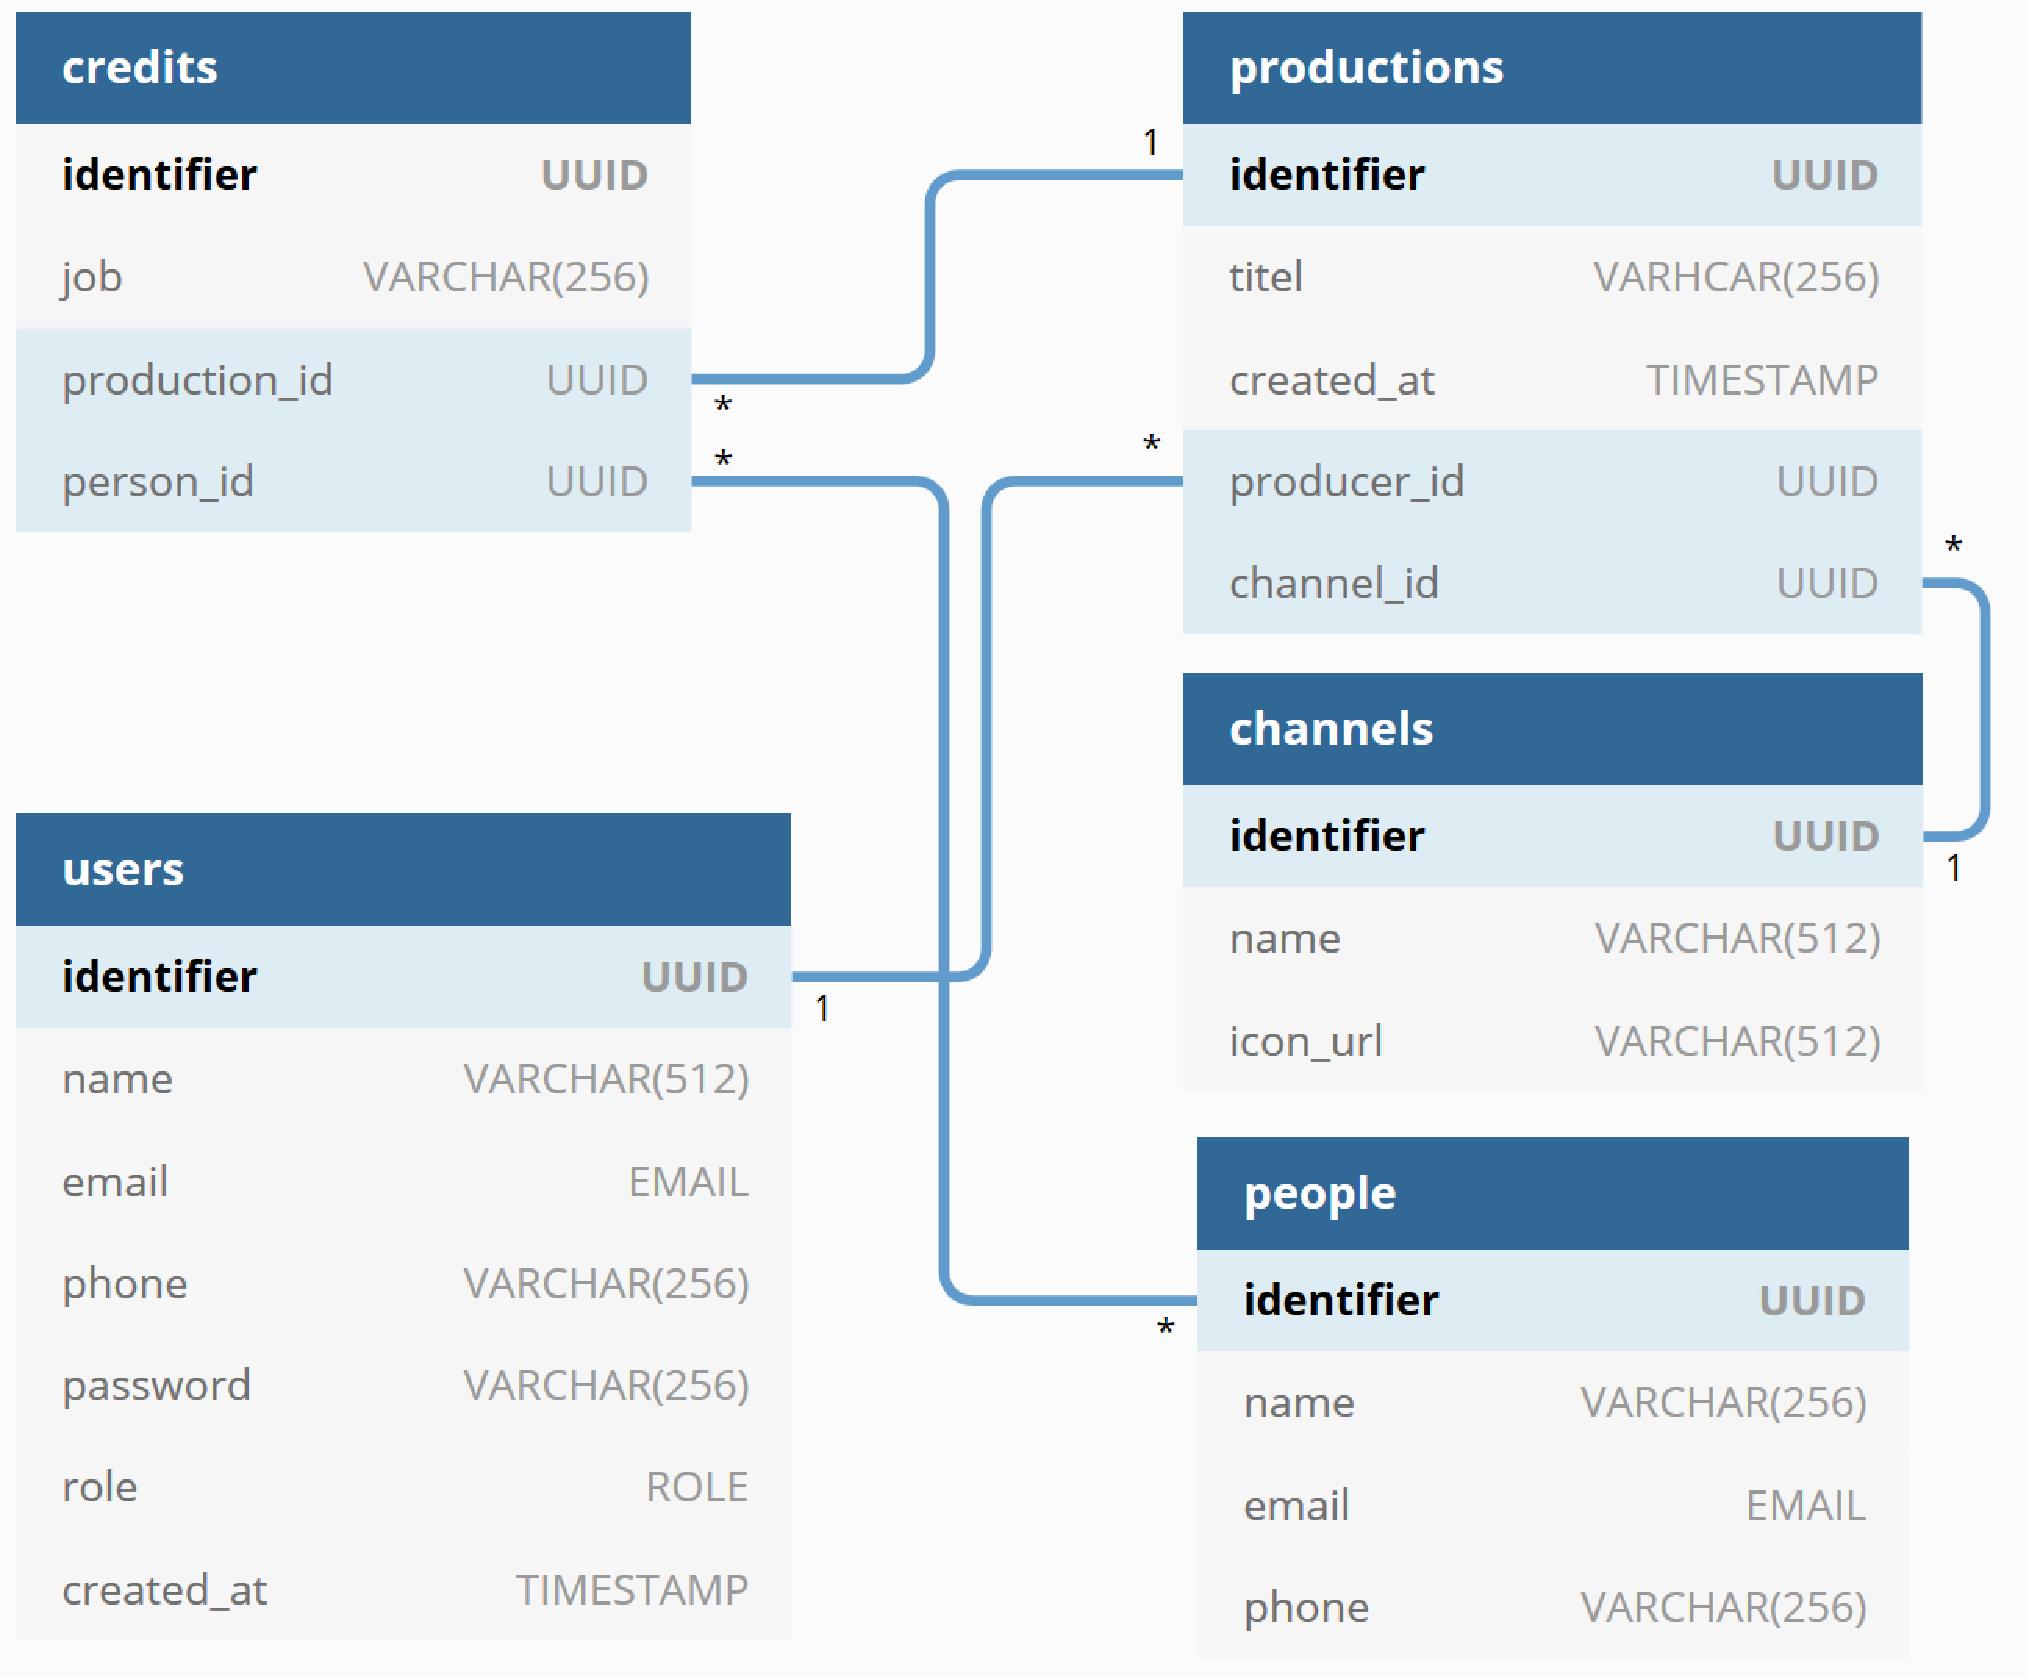
\includegraphics[scale=0.5]{figures/database_design.pdf}  
    \caption{Tabeldesign}
    \label{fig:tabledesign}
\end{figure}{}

% ------------------------------------- channels -------------------------------------
\myparagraph{\texttt{channels}}

% ------ code snippet --------
\begin{lstlisting}[language=sql, caption=channels.sql]
CREATE TABLE channels
(
    identifier UUID NOT NULL,
    name       VARCHAR(512),
    icon_url  VARCHAR(512),
    PRIMARY KEY (identifier)
);
CREATE INDEX channels_name_idx ON channels USING btree (name);
\end{lstlisting}


% ------ table ---------------
\begin{table}[ht]
    \begin{tabularx}{\textwidth}{|X|X|X|}
        \hline
        \texttt{\textbf{identifer}} &  \texttt{\textbf{name}} & \texttt{\textbf{icon\_url}}\\
        \hline
        a4226ce8-e973-4de3-906b-ac4a696c7cdb & TV2 & https://epg-images.tv2.dk/channellogos /logo/3.png \\
        \hline
    \end{tabularx}
    \caption{Tabeldesign: channels}
    \label{tab:channel_table}
\end{table}


% ------------------------------------- users ----------------------------------------
\myparagraph{\texttt{users}}


% ------ code snippet --------
\begin{lstlisting}[language=sql, caption=users.sql]
CREATE EXTENSION citext;
CREATE DOMAIN email AS citext
    CHECK ( value ~
            '^[a-zA-Z0-9.!#$%&''*+/=?^_`{|}~-]+@[a-zA-Z0-9](?:[a-zA-Z0-9-]{0,61}[a-zA-Z0-9])?(?:\.[a-zA-Z0-9](?:[a-zA-Z0-9-]{0,61}[a-zA-Z0-9])?)*$' );
CREATE TYPE role AS ENUM ('royalty_user', 'channel_admin', 'system_admin');
CREATE TABLE users
(
    identifier UUID         NOT NULL,
    name       VARCHAR(512),
    email      email UNIQUE NOT NULL,
    phone      varchar(254),
    password   VARCHAR(256),
    role       role         NOT NULL,
    created_at TIMESTAMP WITH TIME ZONE DEFAULT CURRENT_TIMESTAMP,
    PRIMARY KEY (identifier)
);
CREATE INDEX users_email_idx ON users USING btree (email);
CREATE INDEX users_name_idx ON users USING btree (name);
\end{lstlisting}


% ------ table ---------------
\begin{table}[ht]
    \begin{tabularx}{\textwidth}{|X|X|X|X|X|X|X|}
        \hline
        \texttt{\textbf{identifer}} &  \texttt{\textbf{name}} & \texttt{\textbf{email}} & \texttt{\textbf{phone}} & \texttt{\textbf{password}} & \texttt{\textbf{role}} & \texttt{\textbf{created\_at}}\\
        \hline
        2f477718-3351-4d97-95dd-12518675ed 52 & Simon & string@stri ng.dk & 78652397 & string & 3 & 2020-04-20\\
        \hline
    \end{tabularx}
    \caption{Tabeldesign: users}
    \label{tab:users_table}
\end{table}


% ------------------------------------- people ---------------------------------------
\myparagraph{\texttt{people}}

% ------ code snippet --------
\begin{lstlisting}[language=sql, caption=people.sql]
CREATE TABLE people
(
    identifier UUID NOT NULL,
    phone       VARCHAR(256),
    email      email,
    name       VARCHAR(256),
    PRIMARY KEY (identifier)
);
CREATE INDEX people_name_idx ON people USING btree (name);
\end{lstlisting}



% ------ table ---------------
\begin{table}[ht]
    \begin{tabularx}{\textwidth}{|X|X|X|X|}
        \hline
        \texttt{\textbf{identifer}} &  \texttt{\textbf{name}} & \texttt{\textbf{phone}} & \texttt{\textbf{email}}\\
        \hline
        7fae265e-84d7-4b65-b14e-4ec8819109a7 & Kristian & 42066669 & string2@string2.dk\\
        \hline
    \end{tabularx}
    \caption{Tabeldesign: people}
    \label{tab:people_table}
\end{table}


% ------------------------------------- productions ----------------------------------
\myparagraph{\texttt{productions}}

% ------ code snippet --------
\begin{lstlisting}[language=sql, caption=productions.sql]
CREATE TABLE productions
(
    identifier  UUID         NOT NULL,
    title       VARCHAR(256) NOT NULL,
    created_at  TIMESTAMP WITH TIME ZONE DEFAULT CURRENT_TIMESTAMP,
    producer_id UUID REFERENCES users (identifier),
    channel_id  UUID REFERENCES channels (identifier),
    PRIMARY KEY (identifier)
);
CREATE INDEX production_title_idx ON productions USING btree (title);
CREATE INDEX production_identifier_idx ON productions USING btree (identifier);
\end{lstlisting}

% ------ table ---------------
\begin{table}[ht]
    \begin{tabularx}{\textwidth}{|X|X|X|X|X|}
        \hline
        \texttt{\textbf{identifer}} &  \texttt{\textbf{title}} & \texttt{\textbf{created\_at}} & \texttt{\textbf{producer\_id}} & \texttt{\textbf{channel\_id}}\\
        \hline
        58cb7c91-ed0a-4bd3-80b8-606690441293 & Stuff & 2008-11-11 & 2f477718-3351-4d97-95dd-12518675ed52 &  a4226ce8-e973-4de3-906b-ac4a696c7cdb\\
        \hline
    \end{tabularx}
    \caption{Tabeldesign: productions}
    \label{tab:productions_table}
\end{table}


% ------------------------------------- credits ------------------------------------
\myparagraph{\texttt{credits}}

% ------ code snippet --------
\begin{lstlisting}[language=sql, caption=credits.sql]
CREATE TABLE credits
(
    identifier    UUID         NOT NULL,
    job           VARCHAR(256) NOT NULL,
    production_id UUID REFERENCES productions (identifier),
    person_id     UUID REFERENCES users (identifier),
    PRIMARY KEY (identifier)
);
CREATE INDEX credit_job_idx ON credits USING btree (job);
CREATE INDEX credit_identifier_idx ON credits USING btree (identifier);
\end{lstlisting}


% ------ table ---------------
\begin{table}[ht]
    \begin{tabularx}{\textwidth}{|X|X|X|X|}
        \hline
        \texttt{\textbf{identifer}} &  \texttt{\textbf{job}} & \texttt{\textbf{production\_id}} & \texttt{\textbf{person\_id}}\\
        \hline
        04f699d1-52b6-4eb2-ad88-04f48f93b771 & Lydmand & 58cb7c91-ed0a-4bd3-80b8-606690441293 & 7fae265e-84d7-4b65-b14e-4ec8819109a7\\
        \hline
    \end{tabularx}
    \caption{Tabeldesign: credits}
    \label{tab:credits_table}
\end{table}

\subsubsection{SQL-forespørgelser}
\myparagraph{\texttt{channels}}
\texttt{POST} \texttt{/channels/} der tager \texttt{name} og \texttt{icon\_url} som parametre, og opretter en kanal.\\


\texttt{GET} \texttt{/channels/q} der søger efter alle kanaler, hvor '\texttt{q}' er det parameter der søges efter. Her er det muligt at søge efter navn.\\


\texttt{PATCH} \texttt{/channels/\{channel\_id\}} der opdaterer \texttt{name} og \texttt{icon\_url} på den kanal der tilhører \texttt{channel\_id}\\


\texttt{GET} \texttt{/channels/\{channel\_id\}} der henter den kanal der tilhører \texttt{channel\_id}\\


\texttt{DELETE} \texttt{/channels/\{channel\_id\}} der sletter den kanal der tilhører \texttt{channel\_id}\\


\myparagraph{\texttt{users}}
\texttt{POST} \texttt{/users/} der tager \texttt{name}, \texttt{email}, \texttt{phone}, \texttt{password} og \texttt{repeated\_password} som parametre og opretter en bruger.\\


\texttt{GET} \texttt{/users/q} der søger efter alle brugere, hvor '\texttt{q}' er det parameter der søges efter. Her er det muligt at søge efter navn, email og rolle.\\


\texttt{POST} \texttt{/users/login} der tager \texttt{email} og \texttt{password} som paramtre, og sørger for at en gyldig bruger kan logge ind.\\


\texttt{PATCH} \texttt{/users/\{user\_id\}} der opdaterer en bruger med det valgte \texttt{user\_id}. Det er muligt at opdatere \texttt{name}, \texttt{email}, \texttt{phone} og \texttt{password}.\\


\texttt{GET} \texttt{/users/\{user\_id\}} der henter brugeren med det valgte \texttt{user\_id}.\\


\texttt{DELETE} \texttt{/users/\{user\_id\}} der sletter brugeren med det valgte \texttt{user\_id}.\\


\texttt{PUT} \texttt{/users/\{user\_id\}} tilføjer en bruger med det valgte \texttt{user\_id}. Hvis brugeren allerede eksisterer overskrivers brugeren ellers oprettes der en nu bruger.\\

\myparagraph{\texttt{people}}
\texttt{POST} \texttt{/people/} der tager \texttt{name}, \texttt{email} og \texttt{phone} som parametre og opretter en person.\\


\texttt{GET} \texttt{/people/} der søger efter alle personer, hvor '\texttt{q}' er det parameter der søges efter. Her er det muligt at søge efter navn.\\


\texttt{PATCH} \texttt{/people/\{person\_id\}} der opdaterer en person med det valgte \texttt{person\_id}. Det er muligt at opdatere \texttt{name}, \texttt{email} og \texttt{phone}.\\


\texttt{GET} \texttt{/people/\{person\_id\}} der henter personen med det valgte \texttt{person\_id}.\\


\texttt{DELETE} \texttt{/people/\{person\_id\}} der sletter personen med det valgte \texttt{person\_id}.\\


\texttt{PUT} \texttt{/people/\{person\_id\}} der tilføjer en preson med det valgte \texttt{person\_id}. Hvis personen allerede eksisterer overskrivers personen ellers oprettes der en ny person.\\

\myparagraph{\texttt{productions}}
\texttt{POST} \texttt{/productions/} der tager \texttt{titel}, \texttt{producer\_id} og \texttt{channel\_id} som parametre og opretter en produktion.\\


\texttt{GET} \texttt{/productions/} der søger efter alle produktioner, hvor '\texttt{q}' er det parameter der søges efter. Her er det muligt at søge efter titel og navn og email på producer.\\


\texttt{PATCH} \texttt{/productions/\{production\_id\}} der opdaterer en person med det valgte \texttt{production\_id}. Det er muligt at opdatere \texttt{titel}, \texttt{producer\_id} og \texttt{channel\_id}.\\


\texttt{GET} \texttt{/productions/\{production\_id\}} der henter produktionen med det valgte \texttt{produktion\_id}.\\


\texttt{DELETE} \texttt{/productions/\{production\_id\}} der sletter produktionen med det valgte \texttt{produktion\_id}.\\


\texttt{PUT} \texttt{/productions/\{production\_id\}} der tilføjer en produktion med det valgte \texttt{produktion\_id}. Hvis produktionen allerede eksisterer overskrivers produktionen ellers oprettes der en ny produktion.\\


\myparagraph{\texttt{credits}}
\texttt{POST} \texttt{/credits/} der tager \texttt{job}, \texttt{person\_id} og \texttt{production\_id} som parametre og opretter en kreditering.\\


\texttt{GET} \texttt{/credits/} der søger efter alle krediteringer, hvor '\texttt{q}' er det parameter der søges efter. Her er det muligt at søge efter krediterede personer i det valgte \texttt{production\_id}, efter krediteringer for det valgte \texttt{person\_id} eller efter krediteringer efter det valgte \texttt{job}.\\


\texttt{PATCH} \texttt{/credits/\{credit\_id\}} der opdaterer en person med det valgte \texttt{credit\_id}. Det er muligt at opdatere \texttt{job}, \texttt{person\_id} og \texttt{production\_id}.\\


\texttt{GET} \texttt{/credits/\{credit\_id\}} der henter produktionen med det valgte \texttt{credit\_id}.\\


\texttt{DELETE} \texttt{/credits/\{credit\_id\}} der sletter krediteringen med det valgte \texttt{credit\_id}.\\


\texttt{PUT} \texttt{/credits/\{credit\_id\}} der tilføjer en kreditering med det valgte \texttt{credit\_id}. Hvis krediteringen allerede eksisterer overskrivers krediteringen ellers oprettes der en ny kreditering.\\